% !TeX root = Bachelorarbeit.tex
\chapter{Backend}
\label{Backend}

\section{HomePage}
\label{HomePage}
Die Homepage erscheint zum Start von \emph{Bustracker}, auf dieser Seite wird die Funktion gewählt. Je nach Auswahl wird die entsprechende Page der App geladen.
\subsection{HTML}
Die \gls{gls:html}-Seite in Abb. \ref{fig:Screens} zeigt zwei Buttons, der obere dient dazu das Tracking zu aktivieren und führt auf die \nameref{pag:TrackingPage}. 
Der untere Button dient dazu, ein anderes Gerät zu verfolgen und führt auf die \nameref{pag:WatchPage}.
Am oberen rechten Rand befindet sich ein \glqq Zahnrad\grqq, bei einem Klick darauf erscheint die \nameref{ConfigurationPage}.
\subsection{CSS}

\begin{lstlisting}[float, language=HTML5, caption=Stylesheet für die Homepage , label=lst:HomeCSS]
page-home {
  .scroll-content {
    background-color: #1C4AFF;
  }
  .toolbar-background {
    background-color: #0D47A1;
  }
  .toolbar-title {
    color: white;
  }
  .icon-only {
    background-color: #0D47A1;
  }
  .icon{
      color:white;
    }
  .icon-only{
    background-color: #0D47A1;
    color: #0D47A1;
    }
  .bar-buttons{
    background-color: #0D47A1;
    color: #0D47A1;
  }
}

\end{lstlisting}

Listing \ref{lst:HomeCSS} zeigt das Stylesheet für die Homepage. Die Anweisungen dienen dazu, den Seitenheader in dunkelblau (Hex: 0D47A1) und die Schrift Weiß (Hex: FFFFFF) zu färben.  Der Seitenhintergrund wird mittels der Zeilen 3 - 5 in einem helleren Blau dargestellt (Hex: 1C4AFF).

\subsection{TypeScript}

Die TypeScript Datei \textbf{home.ts} enthält diejenigen Methoden, die nach Betätigen des jeweiligen Buttons die neue Seite aufrufen. Diese sind im Listing \ref{lst:HomeTypescript} zu sehen.

\begin{lstlisting}[float, language=JavaScript, caption= Methoden zur Navigation , label=lst:HomeTypescript]
 goTracking(){
    this.navCtrl.push(TrackingPage).then(()=> console.log('TrackingPage aufgerufen'));
  }

  goWatch(){
    this.navCtrl.push(WatchPage).then(()=> console.log('WatchPage aufgerufen'));
  }

  goConfig(){
    this.navCtrl.push(ConfigPage).then( ()=> console.log('ConfigPage aufgerufen'));
  }
\end{lstlisting}

\section{ConfigurationPage}
\label{ConfigurationPage}
Die Konfigurationsseite (siehe Abb. \ref{fig:Screens}) bietet die Möglichkeit die eigene NutzerID einzustellen. Weiterhin kann die ID des zu trackenden Nutzers eingestellt werden. 
Die API-Aufrufe erfolgen auf der Tracking Seite mit der eigenen ID. Auf der Watchseite wird die ID des zu trackenden Nutzers verwendet.
\subsection{HTML}
Auf der Configuration Page sind zwei Inputs zu sehen. Der erste ist dazu gedacht, die eigene NutzerID einzugeben. Der zweite Input dient zum Eingeben des zu beobachtenden Nutzers.
Es existiert eine \gls{gls:API} Beschränkung. Die IDs müssen existieren, sonst führt dies zu Fehlern bei der Abfrage.
\begin{lstlisting}[float, language=HTML5, caption= Input mittels Databinding , label=lst:ConfigHTML]
 <ion-item>
    <ion-label color="primary" fixed> Eigene ID</ion-label>
    <ion-input type="number" [(ngModel)]="this.rtm.USER_ID" placeholder="Hier ihre eigene ID"></ion-input>
  </ion-item>
\end{lstlisting}
In Listing \ref{lst:ConfigHTML} ist die dynamische Datenbindung zu sehen. Der Nutzer manipuliert den Input, direkt nach der Manipulation wird der Wert in den \nameref{srv:RTMService} gespeichert. Beim Betreten der Seite wird die jeweilige ID direkt aus dem RTMService geladen. 
\subsection{CSS}
\begin{lstlisting}[float, language=HTML5, caption=Stylesheet für die ConfigurationPage , label=lst:ConfigCSS]
page-konfiguration {

.scroll-content {
background-color: #1C4AFF;
}
.toolbar-background {
background-color: #0D47A1;
}
.toolbar-title {
color: white;
}
.bar-button-default-md, .bar-button-clear-md-default, .bar-button-md-default
{
color: white;
}
}
\end{lstlisting}

Listing \ref{lst:ConfigCSS} zeigt das Stylesheet für die Homepage. Die Anweisungen dienen dazu, den Seitenheader in dunkelblau (Hex: 0D47A1) und die Schrift Weiß (Hex: FFFFFF) zu färben. Die Zeilen 12 - 15 dienen dazu, den \glqq Zurück\grqq{}-Pfeil in Weiß einzufärben. Der Seitenhintergrund wird mittels der Zeilen 3 - 5 in einem helleren Blau dargestellt (Hex: 1C4AFF).

\subsection{TypeScript}

In der TypeScript Datei wird der \nameref{srv:RTMService} im Konstruktor instantiiert um das sogenannte \emph{two-way-databinding} zu ermöglichen.  Siehe Listing \ref{lst:ConfigTypeScript}

\begin{lstlisting}[float, language=JavaScript, caption= Konstruktor ConfigurationPage , label=lst:ConfigTypeScript]
 constructor(public navCtrl: NavController, public navParams: NavParams, private rtm: RTMProvider) {}
\end{lstlisting}

\section{TrackingPage}
\label{pag:TrackingPage}

Die TrackingPage (Abb. \ref{fig:Screens}) zeigt die Eigene Position als LatLong Koordinate und als Adresse an. Zusätzlich wird der letzte Checkpoint angezeigt. Über einen Schalter kann der Nutzer das Tracking aktivieren oder deaktivieren.
\subsection{HTML}

Die \gls{gls:html}-Seite der TrackingPage zeigt oben einen Schalter zum Aktivieren oder Deaktivieren des Trackings. Darunter befindet sich ein Feld mit dem Längen- und Breitengrad, sowie die, sich aus dieser Koordinate ergebende Adresse. Die Daten werden via Databinding aus dem \nameref{srv:RTMService} bezogen. Listing \ref{lst:TrackingHTML}

\begin{lstlisting}[float, language=HTML5, caption= Adresse via Databinding , label=lst:TrackingHTML]
<ion-item>
 {{this.rtm._config.lat}}:Latitude {{this.rtm._config.lng}}:Longitude 
 Strasse: {{this.rtm.address.thoroughfare}} Nr: {{this.rtm.address.subThoroughfare}}
  PLZ: {{this.rtm.address.postalCode}} Ort: {{this.rtm.address.locality}}
</ion-item>
\end{lstlisting}


\subsection{CSS}

\begin{lstlisting}[float, language=HTML5, caption=Stylesheet für die TrackingPage , label=lst:TrackingCSS]
page-tracking {
.scroll-content {
background-color: #1C4AFF;
}
.toolbar-background {
background-color: #0D47A1;
}
.toolbar-title {
color: white;
}
.bar-button-default-md, .bar-button-clear-md-default, .bar-button-md-default
{
color: white;
}
}
\end{lstlisting}

Listing \ref{lst:TrackingCSS} zeigt das Stylesheet für die Homepage. Die Anweisungen dienen dazu, den Seitenheader in dunkelblau (Hex: 0D47A1) und die Schrift Weiß (Hex: FFFFFF) zu färben. Die Zeilen 12 - 15 dienen dazu, den \glqq Zurück\grqq{}-Pfeil in Weiß einzufärben. Der Seitenhintergrund wird mittels der Zeilen 3 - 5 in einem helleren Blau dargestellt (Hex: 1C4AFF).

\subsection{TypeScript}

Die TrackingPage instantiiert den \nameref{srv:RTMService}, den \nameref{srv:TrackerService} und den \nameref{srv:iBeaconService}, um auf Werte zugreifen zu können, sowie Methoden der Dienste zu verwenden.


Nachdem die Seite vollständig geladen ist, wird die Funktion \emph{ionViewDidLoad()} ausgeführt. Innerhalb dieser Funktion wird der Status des \glqq trackingIndicators \grqq abgefragt, basierend darauf wird das Tracking gestartet oder gestoppt. Dazu kommt eine If-Abfrage in Form eines bedingten ternären Operators zum Einsatz \cite{TernärerOperator}.  Siehe Listing \ref{lst:TrackingTypescript}. 

\begin{lstlisting}[float, language=JavaScript, caption= ionViewDidLoad()-Methode der TrackingPage , label=lst:TrackingTypescript]
 ionViewDidLoad() {
    console.log('ionViewDidLoad TrackingPage');
    (this.rtm.trackingIndicator.valueOf()== true) ? this.trackerService.startTracking() : this.trackerService.stopTracking();
    console.log(this.rtm.trackingIndicator.valueOf());
    this.beaconService.initBeacon();
}
\end{lstlisting}

Im Anschluss wird der \nameref{srv:iBeaconService} gestartet. Beim Verlassen der Seite wird automatisch der Inhalt vom \nameref{srv:RTMService} auf den Festspeicher übertragen.

\section{WatchPage}
\label{pag:WatchPage}

Die WatchPage zeigt die Position des beobachteten Geräts auf einer Karte, als LatLong-Koordinate und als Adresse an.

\subsection{HTML}

Die WatchPage (Abb. \ref{fig:Screens}) zeigt eine GoogleMaps-Karte mit Positionsinformationen des zu beobachtenden Nutzers an. Die Karte stellt der \nameref{MapsService} bereit. Sie wird an das \emph{div} mit dem Namen 
\glqq map\_canvas\grqq{} gebunden.
Zusätzlich ist die aktuelle Adresse der Position und der letzte Checkpoint zu sehen.
Adresse und Checkpoint werden hier analog zur \nameref{pag:TrackingPage} vom \nameref{srv:RTMService} zur Verfügung gestellt und angezeigt.

\subsection{CSS}

Die Google Karte benötigt einen transparenten Hintergrund und ein benanntes <div>. Hier wird die Karte in einer sogenannten ion-card angezeigt, einem Template des Ionic-Frameworks. Mittels \gls{gls:css} wird diese Card als transparent gekennzeichnet. Listing \ref{lst:WatchCSS} zeigt die Style-Konfiguration für das <div> und die Klasse \glqq transparent-card\grqq{}. Zusätzlich sind die Stylingoptionen für sichtbare \gls{gls:css}-Elemente eingetragen, analog zu den anderen Seiten um das Erscheinungsbild möglichst einheitlich zu gestalten.

\begin{lstlisting}[float, language=HTML5, caption= Transparentes Canvas und Styling der WatchPage, label=lst:WatchCSS]
page-watch {
  #map_canvas {
    height: 90%;
  }
  .transparent-card{
    background-color: transparent;
  }
  .scroll-content {
  background-color: #1C4AFF;
  }
  .toolbar-background {
  background-color: #0D47A1;
  }
  .toolbar-title {
  color: white;
  }
  .bar-button-default-md, .bar-button-clear-md-default, .bar-button-md-default
  {
  color: white;
  }
}
\end{lstlisting}

\subsection{TypeScript}

Die WatchPage verfügt, analog zur \nameref{pag:TrackingPage}, über eine \emph{ionViewDidLoad()}-Methode. In dieser wird der \nameref{MapsService} initialisiert. 
Die Seite bietet verschiedene Methoden zum Abrufen und Zeichnen der Position des gewünschten Teilnehmers. Listing \ref{lst:WatchTypeScript} zeigt die Methode zum Abrufen der letzten Position eines Teilnehmers.



\begin{lstlisting}[float, language=JavaScript, caption=Methode zum Abruf der letzten Position , label=lst:WatchTypeScript]
getSinglePos(){
  this.apiService.getLastLocationById(this.rtm.trackingID).then(
    (data)=> {
    this.rtm.lat = data.lat;
    this.rtm.long = data.lon;
    this.trackerService.geoCode();
  }).catch((err)=> {console.log('Fehler getSinglePos: ' + JSON.stringify(err))});
}
\end{lstlisting}


\begin{figure}[htbp] 
	\centering
	
\includegraphics[width=0.35\textwidth]{images/Homepage.png}
	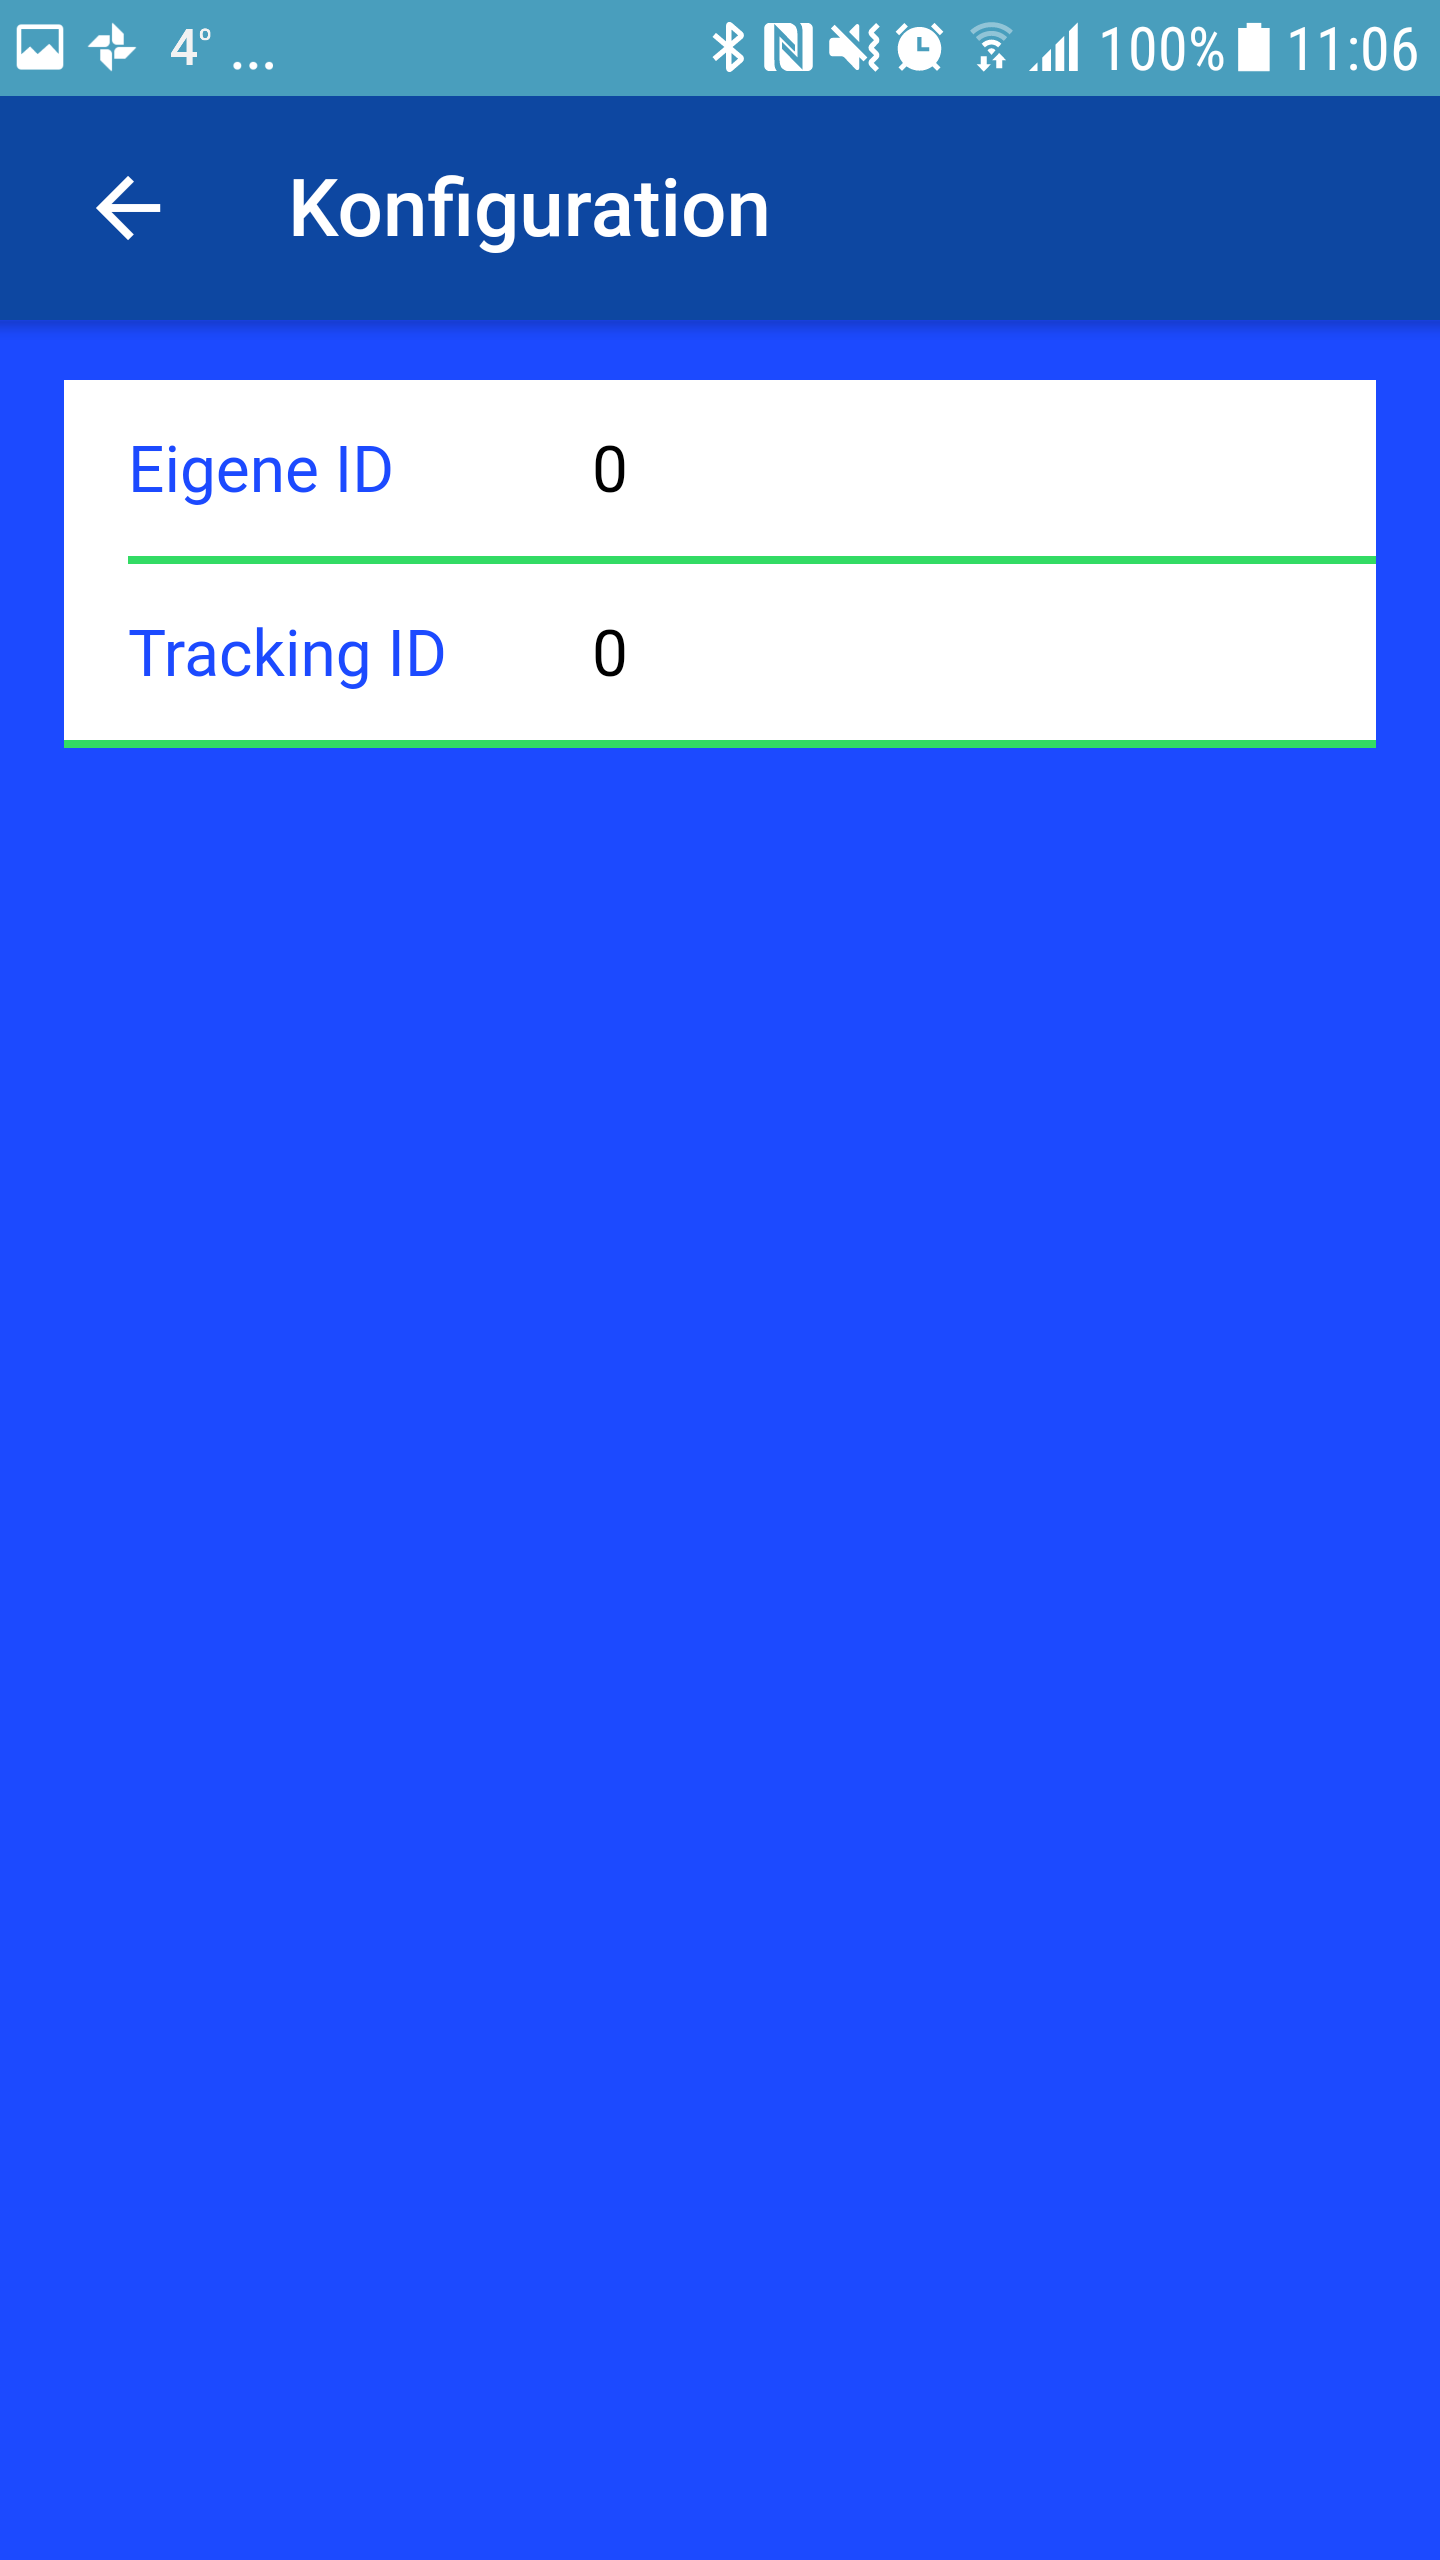
\includegraphics[width=0.35\textwidth]{images/Configpage.png}
	\caption{Home-  und Configpage von \emph{Bustracker}}
	\label{fig:Screens}
\end{figure}
\begin{figure}[htbp]
	\centering
	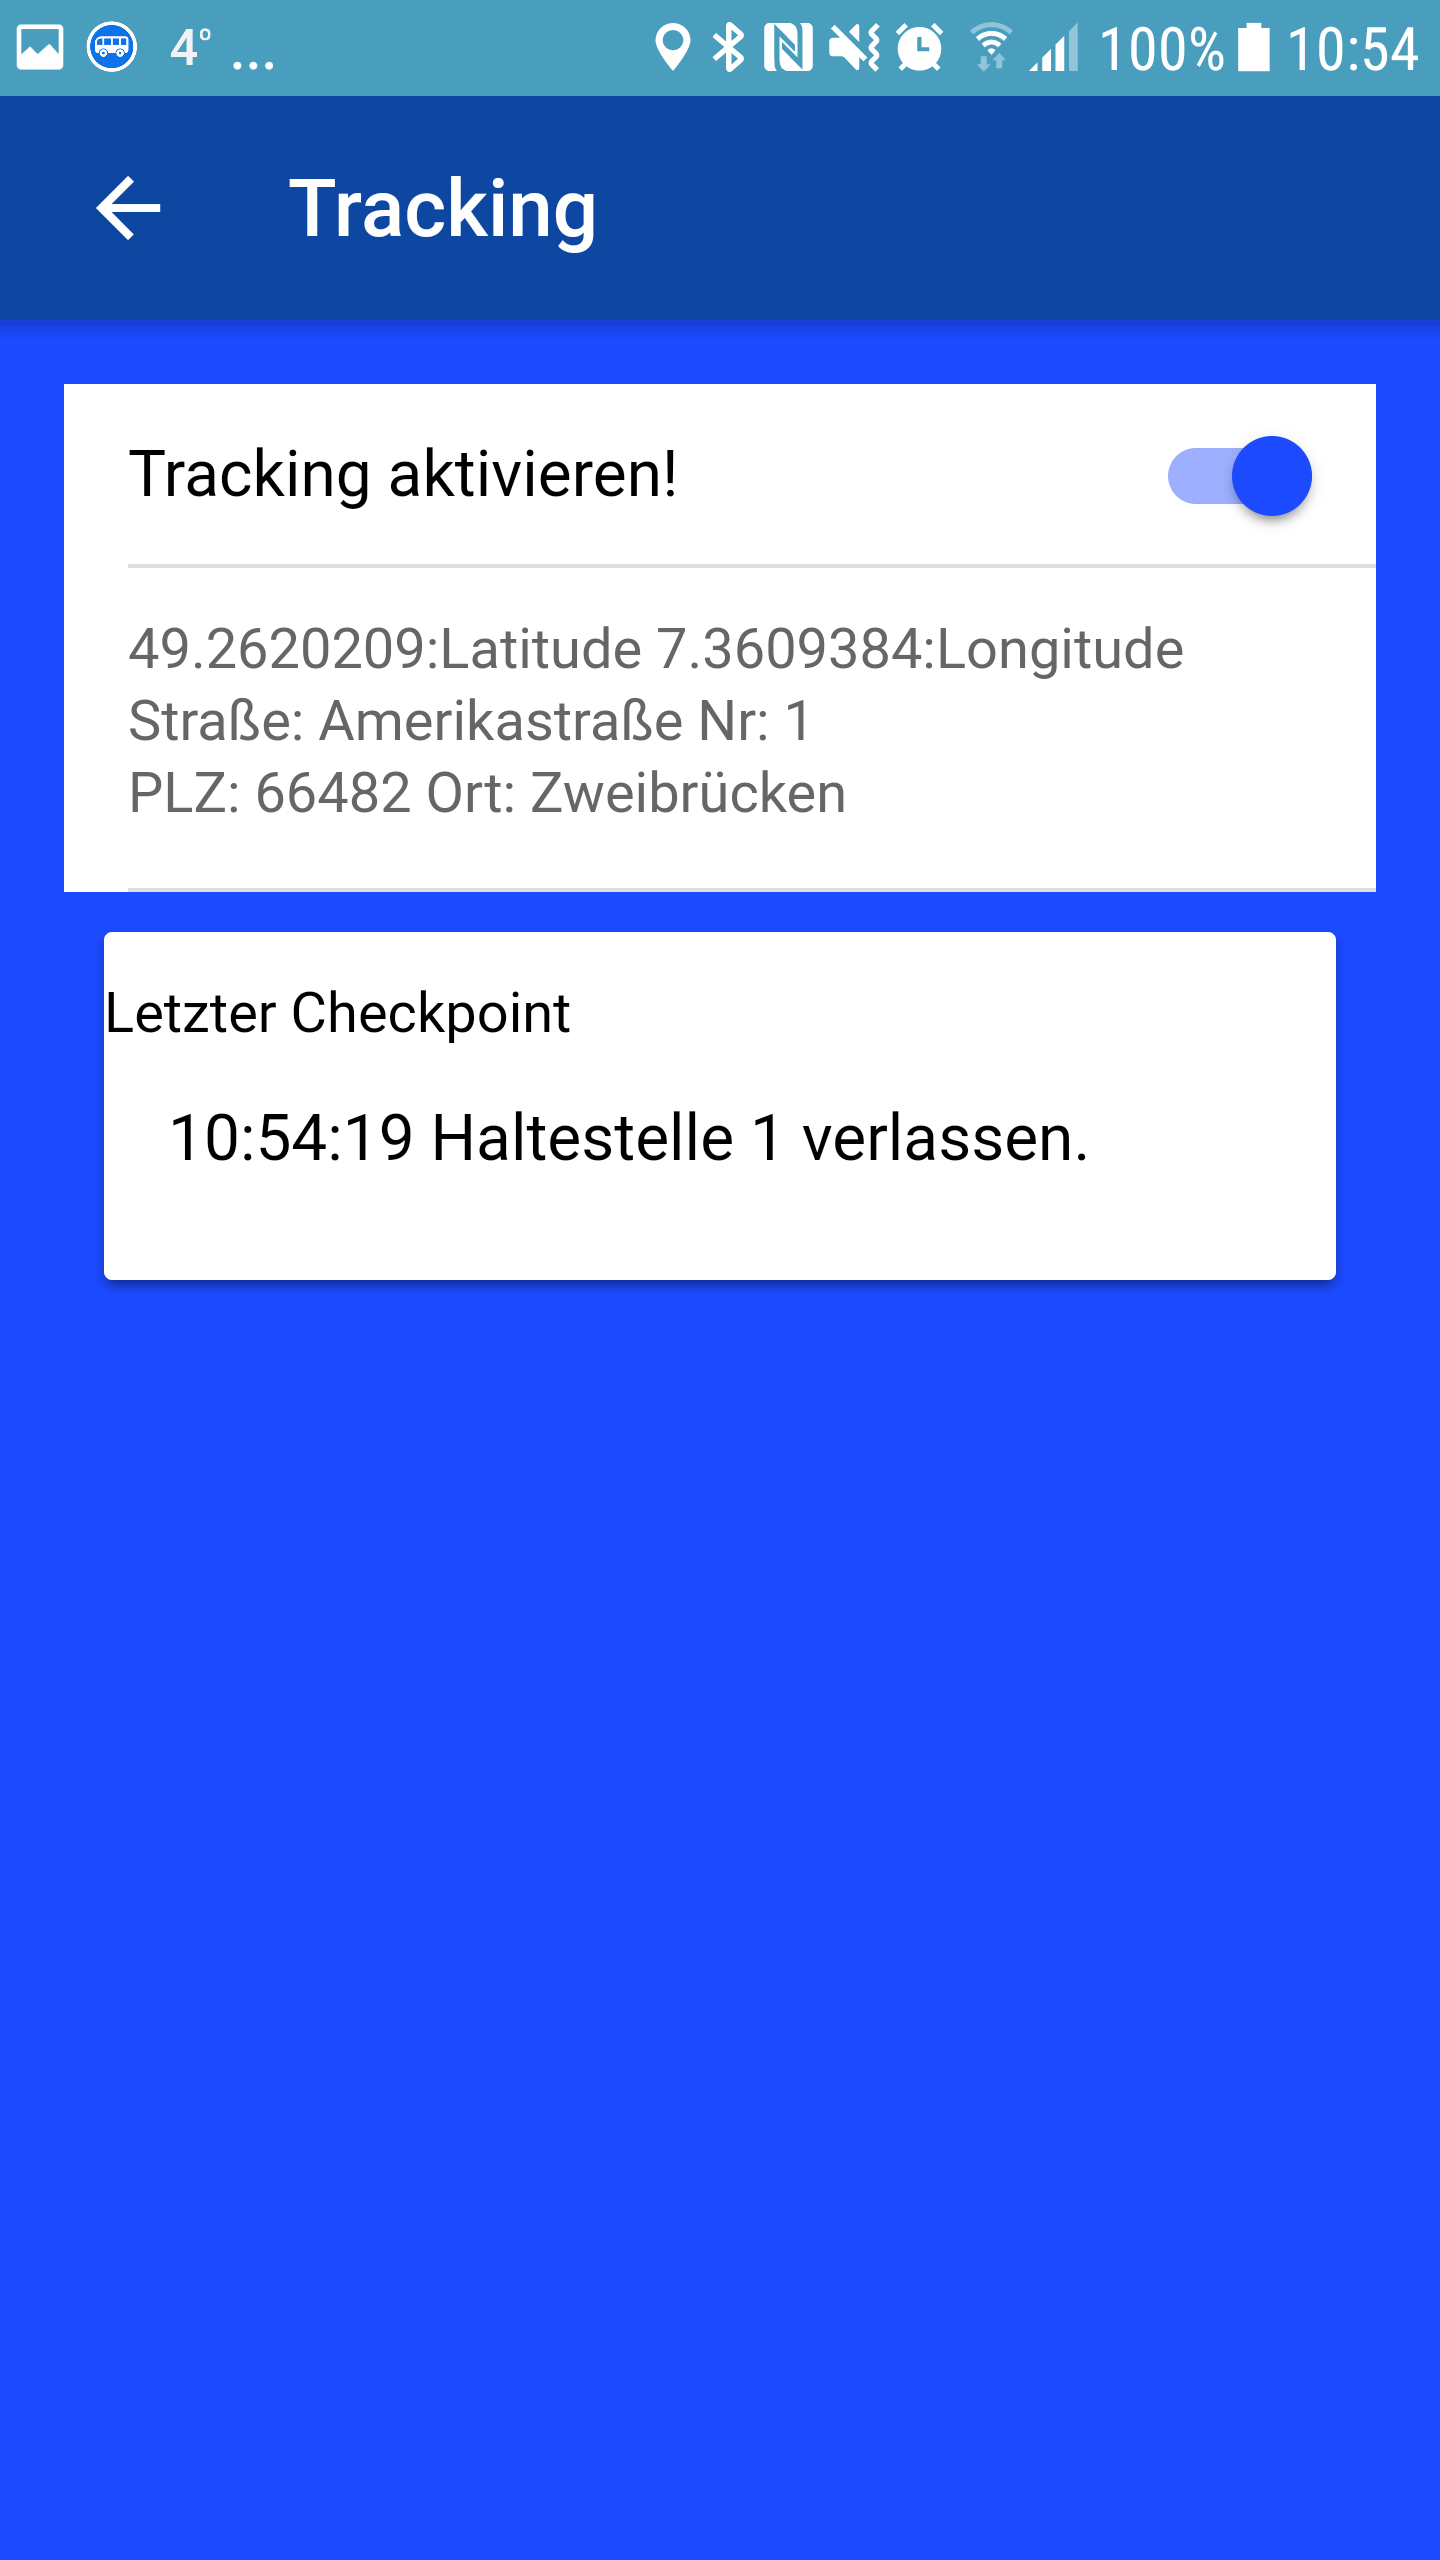
\includegraphics[width=0.35\textwidth]{images/Trackingpage.png}
	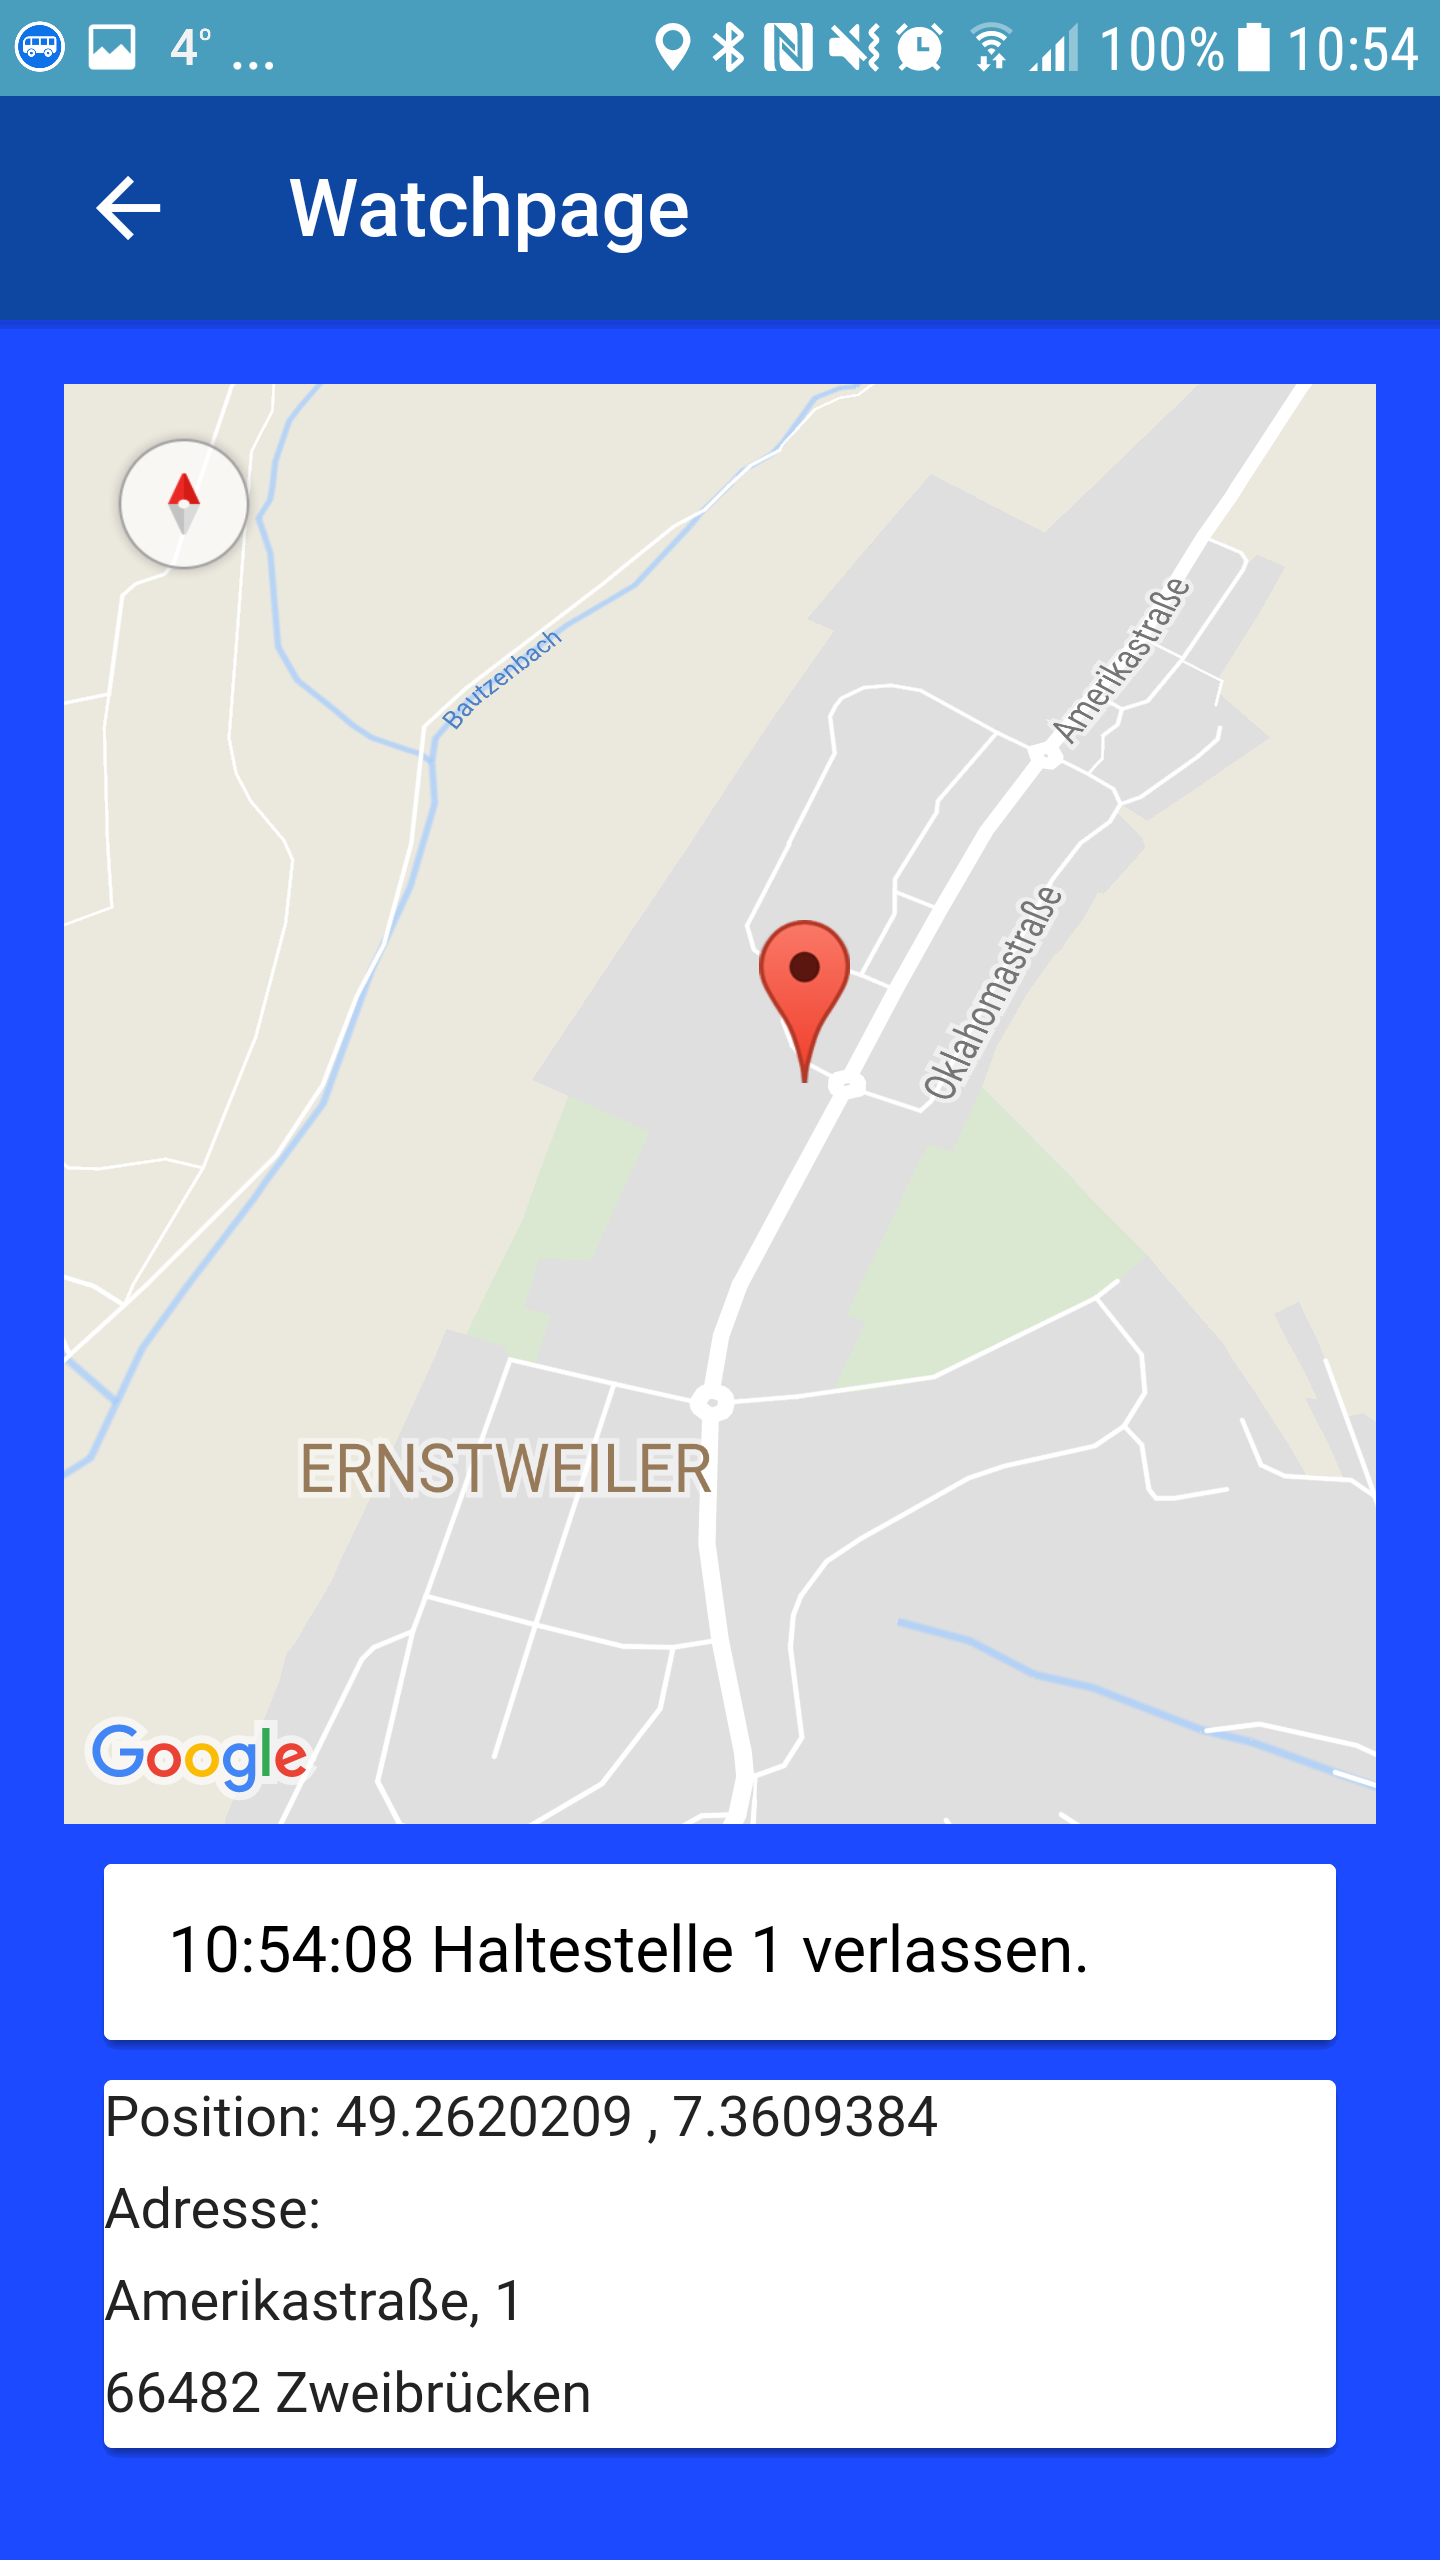
\includegraphics[width=0.35\textwidth]{images/Watchpage.png}
	\caption{Tracking- und Watchpage von \emph{Bustracker}}
\end{figure}

\pagebreak
\section{APIService}
\label{srv:APIService}
Der \gls{gls:API} Service übernimmt die Kommunikation mit der \gls{gls:rest}-\gls{gls:API} von \emph{Bustracker}. 
\subsection{Verwendete Plugins}
@angular/common/http \cite{AngularHttp}
\subsection{Arbeitsweise}
Der Service stellt eine \textbf{POST} Methode bereit, mit der die Daten des Mobilgeräts  an die API gesendet werden. Diese Funktion kommt beim Tracking \ref{srv:TrackerService} zum Einsatz.
Das Abrufen der Daten geschieht mittels verschiedener \textbf{GET} Methoden. Es können alle gespeicherten oder die letzte gespeicherte Position eines mittels \textbf{ID}{} festgelegten Teilnehmers abgerufen werden. Listing \ref{lst:APIService}.

\begin{lstlisting}[float, language=JavaScript, caption= Rückgabe aller gültigen Positionsdaten der jeweiligen TrackingID , label=lst:APIService]
getAllDataById(id: number) {
    console.log('GET URL: ' + this.rtm.URL + '/' + id);
    this.http.get(this.rtm.URL + '/' + this.rtm.trackingID, {headers: this.headers}).subscribe(
      (data) => {
        data['result'].forEach((itr) => {
          this.rtm.trackPoints.push(itr);
          console.log(JSON.stringify(itr))
        });
        this.apiCallID = data;
        },
      (err) => {
        console.log('Fehler beim get-Request' + JSON.stringify(err));
      });
    }
\end{lstlisting}

\section{iBeaconService}
\label{srv:iBeaconService}
Der iBeaconService verwaltet Events, die durch das Betreten oder Verlassen des Sendebereichs eines iBeacons ausgelöst werden.
\subsection{Verwendete Plugins}
@ionic-native/ibeacon \cite{iBeaconPluginDoku}
\subsection{Arbeitsweise}
\emph{Bustracker} hört auf zwei Ereignisse, das Betreten und Verlassen des Sendebereichs eines Beacons. Die Beacons sind zwar aktive Sender, jedoch ändern diese ihr Verhalten nicht wenn ein Ereignis eintritt.
Vereinfacht kann man sagen, iBeacons transferieren ortsbezogene Ereignisse in eine Art, die durch Software erfassbar ist und somit auf diese Ereignisse reagiert werden kann. 
Befindet sich ein iBeacon in Reichweite des Gerätes, so wird dieses erkannt und mit bekannten iBeacons verglichen. Im Erfolgsfall, also das Beacon ist der Software bekannt, wird eine Benachrichtigung auf dem Gerät angezeigt, die  Checkpointanzeige aktualisiert und der Checkpoint der \gls{gls:API} mitgeteilt.

Beim Verlassen des Sendebereichs wird ebenfalls eine Meldung (siehe \nameref{srv:LNotificationService}) angezeigt, der Checkpoint Status (siehe \nameref{pag:WatchPage}) aktualisiert und die \gls{gls:API} (siehe \nameref{srv:APIService}) wird informiert.

	\begin{figure}[htbp] 
  \centering
     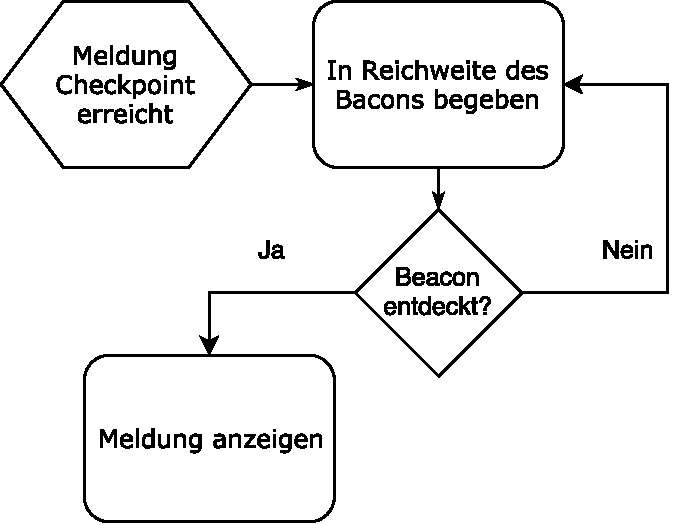
\includegraphics[width=0.5\textwidth]{images/beaconflowchart.pdf}
  \caption{Einsatz eines iBeacons als Flussdiagramm}
  \label{fig:Beaconflowchart}
\end{figure}

Der iBeaconService stellt die Funktionen zum \glqq Hören\grqq auf iBeacons bereit. Zuerst wird ein Delegat \cite{Schatten2010} für den nativen LocationManager erzeugt. Im Anschluss wird sich bei den benötigten EventListenern des Delegaten registriert. Die EventListener sind als Observeables ausgeführt, somit ist es einfach Zustandsänderungen zu detektieren. Listing \ref{lst:ExitRegion} zeigt eine solche Registrierung und die im Erfolgsfall (also hier das Verlassen einer Region) auszuführenden Funktionsaufrufe.

\begin{lstlisting}[float, language=JavaScript, caption= Registrieren beim didExitRegion-EventListener  , label=lst:ExitRegion]
delegate.didExitRegion()
      .subscribe(
      (data) =>{
          this.notificationService.updateWaypoint(data.region.identifier);
        console.log('Gebiet verlassen: ', data.region.identifier);}      
      );
\end{lstlisting}

Die zu entdeckenden Regionen müssen mitgeteilt werden. Dazu verwendet man eine Methode der lokalen Instanz des Plugins. Diese Methode \textit{startMonitoringForRegion(beacon : BeaconRegion)} ist als Promise ausgeführt, da sie asynchron ist. Es ist möglich, den Erfolgs- oder Fehlerfall abzufragen, so dass es eine Mitteilung gibt, wenn die Region nicht beobachtet werden kann. 

\begin{lstlisting}[float, language=JavaScript, caption= Übergabe einer Region an das iBeacon Objekt.  , label=lst:RegisterRegion]
let beacon1 = this.iBeacon.BeaconRegion('Haltestelle 1' , this.rtm.UUID, 10001, 10002);
.
.
.
this.iBeacon.startMonitoringForRegion(beacon1)
       .then(
         (data) => console.log('Native layer received the request to monitoring' + JSON.stringify(data)),
         error => console.error('Native layer failed to begin monitoring: ', JSON.stringify(error))
       );
\end{lstlisting}

  
\section{Local Notification Service}
\label{srv:LNotificationService}
Der Local Notification Service dient dazu Statusinformationen über die jeweiligen Checkpoints als Mitteilung auf dem Bildschirm oder im Notificationcenter eines Smartphone anzuzeigen.
\subsection{Verwendete Plugins}
@ionic-native/local-notification \cite{LocalNotificationPluginDoku}
\subsection{Arbeitsweise}
 Die Nachricht enthält die Uhrzeit und den Checkpoint sowie den Status erreicht bzw. verlassen. Abbildung \ref{fig:Notification} zeigt eine solche Notification.
 
\begin{figure}[htbp] 
  \centering
     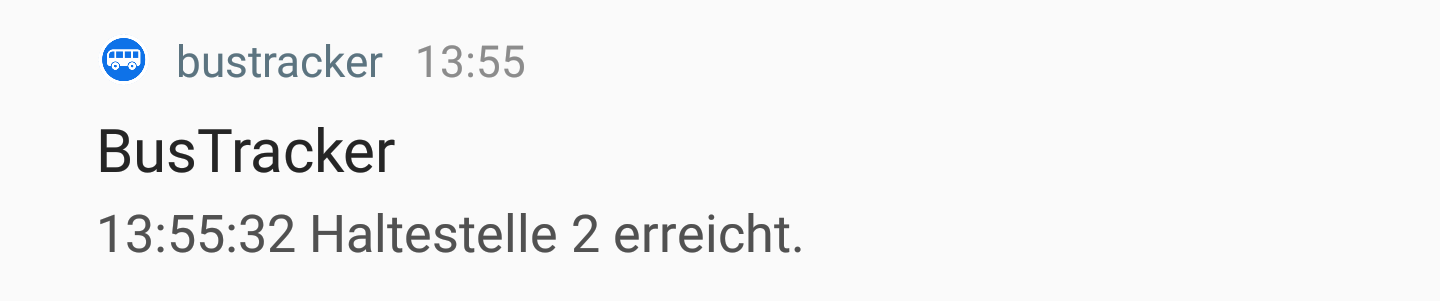
\includegraphics[width=0.5\textwidth]{images/Notification.png}
	   \caption{Benachrichtigung im Notification Center}
  \label{fig:Notification}
\end{figure}

Das Erzeugen einer Notification ist in Listing \ref{lst:ScheudleNotification} dargestellt. Basierend auf dem Namen des iBeacons wird die Nachricht generiert. Die \emph{.schedule()}-Methode lässt die Nachricht im Notification Center des Telefons erscheinen.

\begin{lstlisting}[float, language=JavaScript, caption= Erzeugen einer Notification bei Erreichen einer Haltestelle , label=lst:ScheudleNotification]
sendWaypointNotification(identifier: string ){
    let text: string = '';
    text = this.rtm.timeHelper(); switch(identifier){
      case 'Haltestelle 1':{ text = text + ' Haltestelle 1 erreicht.';
                              this.rtm.LOGARRAY.push(text);
                              break;}
      case 'Haltestelle 2':{ text = text + ' Haltestelle 2 erreicht.';
                              this.rtm.LOGARRAY.push(text);
                              break;}
      case 'Haltestelle 3':{ text = text + ' Haltestelle 3 erreicht.';
                              this.rtm.LOGARRAY.push(text);
                              break; }
      default: {text = 'Ein Beacon wurde nicht zugeordnet.'};

    }

    this.notification.schedule({id: 1, title:'BusTracker', text: text, led:'#FF0000'});
  }
\end{lstlisting}

Listing \ref{lst:UpdateNotification} zeigt den Aktualisierungsprozess der Notification. Basierend auf dem Beaconnamen wird die Notification aktualisiert.

\begin{lstlisting}[float, language=JavaScript, caption= Update einer Notification bei Verlassen einer Haltestelle , label=lst:UpdateNotification]
updateWaypoint(identifier : string){
    let text: string = '';
    text = this.rtm.timeHelper();
    switch(identifier){
      case 'Haltestelle 1':{ text =  text + ' Haltestelle 1 verlassen.';
                              this.rtm.LOGARRAY.push(text);
                              break;}
      case 'Haltestelle 2':{ text =  text + ' Haltestelle 2 verlassen.';
                              this.rtm.LOGARRAY.push(text);
                              break;}
      case 'Haltestelle 3':{ text =  text + ' Haltestelle 3 verlassen.';
                              this.rtm.LOGARRAY.push(text);
                              break;}
 		 default: {text = 'Update, kein gueltiger case' };
    }
    this.notification.update({id: 1, text: text, led:'#FF0000'});
  }
\end{lstlisting}



\section{LoadService}
\label{srv:LoadService}
Der LoadService dient zum Laden gespeicherter Werte vom Festspeicher des Telefons in den Laufzeitspeicher \nameref{srv:RTMService}.
\subsection{Verwendete Plugins}
keine 
\subsection{Arbeitsweise}
Die Methoden des LoadService rufen Methoden des \nameref{srv:PersistenzService} auf. Die Rückgabewerte des LoadService sind als Promises ausgeführt, da die Festspeicherzugriffe asynchron erfolgen. 

Listing \ref{lst:LoadUserID} dient als Beispiel und zeigt die Methode um die UserID zu laden. Sie ruft eine Methode des \nameref{srv:PersistenzService} auf, wartet auf das Ergebnis und gibt dieses dann zurück.
  
\begin{lstlisting}[float, language=JavaScript, caption= Laden der UserID , label=lst:LoadUserID]
loadUserID(): Promise<number>{
    console.log('LoadService: LoadUSERID');
    return this.persist.loadUserID();
  }
  \end{lstlisting}
  
\section{SaveService}
\label{srv:SaveService}
Der SaveService hat die Aufgabe, Daten und Werte aus dem Laufzeitspeicher \nameref{srv:RTMService} in den Festspeicher \nameref{srv:PersistenzService} zu überführen.
\subsection{Verwendete Plugins}
keine
\subsection{Arbeitsweise}
Es wird eine im PersistenzSerivce \ref{srv:PersistenzService} vorhandene generische Speichermethode mit Übergabeparametern aufgerufen. Listing \ref{lst:SaveUserID} zeigt den Aufruf. Die Methode des \ref{srv:PersistenzService} ist generisch, so müssen als Argumente ein Label vom Typ String und ein Parameter, hier vom Typ number übergeben werden.

\begin{lstlisting}[float, language=JavaScript, caption= Speichern der UserID , label=lst:SaveUserID]
saveUserID(uid: number){
    console.log('SaveService: UserID');
    this.persistenzService.saveSingleParameter('USERID', uid);
  }
\end{lstlisting}

\section{PersistenzService}
\label{srv:PersistenzService}
Der PersistenzService verwaltet den Festspeicher des Geräts und bietet dafür Lade- und Speichermethoden an.
\subsection{Verwendete Plugins}
@ionic-native/native-storage \cite{NativeStoragePluginDoku}
\subsection{Arbeitsweise}
Der Speicher wird \glqq Native Storage \grqq genannt. Es wird der native Speicher des jeweiligen Geräts verwendet. Das Speichern erfolgt via Key und Value. Soll nun ein Wert geladen werden, so wird die entsprechende \textit{Load}-Methode mit dem Key aufgerufen. Im Beispiel \ref{lst:LoadUserIDPersist} wird die UserID vom Festpeicher geladen. Der Zugriff erfolgt asynchron. Die UserID wird als Promise zurückgegeben.

\begin{lstlisting}[float, language=JavaScript, caption= Laden der UserID vom Native Storage, label=lst:LoadUserIDPersist]
loadUserID(): Promise<number> {
    console.log('PersistenzService: LoadUserID');
    return this.nstorage.getItem('USERID');
  }
\end{lstlisting}

Soll ein Wert gespeichert werden, so kommt die generische Speichermethode zum Einsatz. Hier wird schon wie im \nameref{srv:SaveService} Referenz und Wert übergeben. Die Methode \emph{setItem} ist als
Promise ausgeführt, um der Asynchronität Rechnung zu tragen. 

\begin{lstlisting}[float, language=JavaScript, caption=Generische Speichermethode für Native Storage, label=lst:SaveGeneric]
saveSingleParameter(ref:string, value:any) {
    console.log('PersistenzService: save');
    this.nstorage.setItem(ref, value).then(() =>
      console.log(ref + 'gespeichert!'), (err) => {
      console.log('Fehler beim Speichern von ' + ref + '' + JSON.stringify(err));
    })
  }
\end{lstlisting}

\section{RTMService}
\label{srv:RTMService}
Der Laufzeitspeicher enthält die Daten und Werte, die zur Laufzeit benötigt werden.
\subsection{Verwendete Plugins}
@ionic-native/native-geocoder \cite{GeocoderPluginDoku}
\subsection{Arbeitsweise}
Der RTMService nimmt Werte von verschiedenen  Services entgegen und stellt sie anderen Services zur Verfügung. Alle Dienste die Daten anliefern oder benötigen, instanzieren den RTMService. Die Services, die Speicher- oder Lademethoden benötigen, rufen diese ebenfalls über den RTMService auf.  

\begin{lstlisting}[float, language=JavaScript, caption=Methode zum Persistieren des Appzustandes beim Beenden, label=lst:saveAll]
save(){
    console.log('RTM SaveMethode aufgerufen.')
    this.saveService.saveTrackingIndicator(this.trackingIndicator);
    this.saveService.saveURL(this.URL);
    this.saveService.saveLat(this.lat);
    this.saveService.saveLong(this.long);
    this.saveService.saveADDRESS(this.address);
    this.saveService.saveTrackMarkers(this.trackMarkers);
    this.saveService.saveUserID(this.USER_ID);
    this.saveService.saveTrackingCode(this.trackingCode);
    this.saveService.saveLOGARRAY(this.LOGARRAY);
    this.saveService.saveTrackingID(this.trackingID);
    this.saveService.saveUUID(this.UUID);
  }
\end{lstlisting}


\section{MapsService}
\label{MapsService}
Der MapsService dient zur Darstellung der Eigen- und Fremdposition auf einer Karte. Hier wird auch der zurückgelegte Weg des Beobachteten angezeigt.
 
\subsection{Verwendete Plugins}
@ionic-native/google-maps \cite{GoogleMapsPluginDoku}
\subsection{Arbeitsweise}
Der MapsService bietet unter Verwendung der GoogleMaps \gls{gls:API} die Möglichkeit Dinge auf einer Karte darstellen zu lassen.
Der MapsService erzeugt eine Karte, die zuvor durch Optionen parametriert wird. In Listing \ref{lst:GoogleMapConfig} ist die Instantiierung der Karte dargestellt.

\begin{lstlisting}[float, language=JavaScript, caption= Instantiierung GoogleMap, label=lst:GoogleMapConfig]
this._map = GoogleMaps.create('map_canvas', {
 camera: {
   target: {
     lat: 49.26204150113853,
     lng: 7.36005587579744
   },
  zoom: 15,
  tilt: 30
  }
});
\end{lstlisting}

Die hier angegebenen Optionen sind \emph{map\_canvas}, der Name des <div> in dem die Karte erscheinen soll, und die Position der Kamera. Die Kameraposition wird hier als \emph{target} bezeichnet und enthält einen Längen- sowie einen Breitengrad als Koordinate. Weitere Kameraoptionen sind \emph{zoom}, die Größe des sichtbaren Ausschnitts und \emph{tilt} die Neigung. 

Nachdem die Karte geladen wurde, wird mittels der \emph{.one}-Methode einmalig auf ein Event gewartet. In dieser Situation wird auf das \textbf{MAP\_READY}-Event gewartet. Die \emph{.one}-Methode ist als Promise ausgeführt. Wenn die Karte bereit ist, wird das \emph{mapReady}-Flag auf true gesetzt und die eigene Position abgefragt. Basierend auf den Positionsdaten wird mit \glqq \emph{return this.\_map.addMarker() .. }\grqq{}
eine Markierung auf die Karte gesetzt. Diese Markierung muss ebenfalls parametriert werden. 

Die Optionen sind: 
\begin{description}
\item \textbf{title} Titel bzw. Name des Markers.
\item \textbf{snippet} Zusatztext, der nach dem Klicken auf den Marker angezeigt wird.
\item \textbf{position} Position des Markers als LatLong-Koordinate.
\item \textbf{animation} Animation, mit der der Marker an der in \emph{position} angegebenen Stelle auftaucht.
\end{description}

Der dazugehörige Programmcode befindet sich in Listing \ref{lst:GoogleMapPosition}.


\begin{lstlisting}[float, language=JavaScript, caption=Automatische Darstellung der eigenen Position, label=lst:GoogleMapPosition]
this._map.one(GoogleMapsEvent.MAP_READY).then(() => {
this._mapReady = true;
this._map.getMyLocation().then((location: MyLocation) =>{
return this._map.addMarker({
title: 'Sie sind hier!',
snippet: 'Ihre aktuelle Position',
position: location.latLng,
animation: GoogleMapsAnimation.BOUNCE
})})
});
}
\end{lstlisting}

\section{TrackerService}
\label{srv:TrackerService}

Der Location Tracker stellt die aktuelle \gls{gls:gps} Position des Telefons bereit und überträgt diese an den \nameref{srv:RTMService}. 
Das Ermitteln der \gls{gls:gps} Position ist nicht immer gleich, es wird unterschieden ob sich die Anwendung im Vorder- oder Hintergrund befindet.
\subsection{Verwendete Plugins}
@ionic-native/BackgroundGeolocation \cite{bGeolocation}

@ionic-native/Geolocation \cite{Geolocation}
\subsection{Arbeitsweise}
Sobald der Nutzer auf der Homepage \textbf{Tracking} auswählt, wird die Positionserfassung mittels \textit{startTracking()} gestartet. Nachdem eine Positionsfeststellung erfolgt ist, wird die Position mithilfe des \nameref{srv:APIService} an die \gls{gls:API} weitergegeben. 

Beim Aufruf der Seite wird der  \nameref{srv:iBeaconService} mittels der Methode \textbf{initBeacon()} aktiviert und iBeacons werden nun erkannt.
 
\subsubsection*{Hintergrund}

Wird \emph{Bustracker} in den Hintergrund geschickt, ist das Hintergrundtracking aktiv. Dies geschieht regelmäßig bei der Nutzung einer anderen App oder beim Deaktivieren des Bildschirms. 
Das backgroundGeolocation-Plugin benötigt eine Konfiguration. Diese wird im Code direkt vor dem Aufruf der eigentlichen Methode erzeugt.
\begin{lstlisting}[float, language=JavaScript, caption= Konfiguration Backgroundtracking, label=lst:BTConf]
 let config = {
            desiredAccuracy: 0,
            stationaryRadius: 20,
            distanceFilter: 10,
            debug: false,
            interval: 1000,
            startForeground: false
            stopOnTerminate: true,
        };
\end{lstlisting}

Diese Konfiguration wird an die \emph{.configure()} Methode übergeben, diese liefert ein Observeable vom Typ \emph{BackgroundGeolocationResponse} zurück. 

Das Backgroundtracking wird mittels der \emph{.configure()} Methode konfiguriert und muss explizit durch die \emph{.start()} Methode aktiviert werden. Die \emph{.start()} Methode gibt ein Promise zurück, ob das Starten geglückt ist. Im Erfolgsfall, kann mit \emph{.then(()=>{})} weiterer Code ausgeführt werden, der auf den erfolgreichen Start wartet. Der Fehlerfall kann mittels \emph{.catch((err)=>{})} abgefangen werden. 

Die BackgroundGeolocationResponse wird im angegebenen Intervall (Millisekunden) aktualisiert. Bei \emph{Bustracker} werden aktuell Längen- und Breitengrad als Datum im Latlong- Format verwendet. Diese können vom \emph{location}-Objekt mittels Punktoperator gewonnen werden. Die Verwendung wird in Listing \ref{lst:BTAufruf} gezeigt. Jede Aktualisierung stellt einen Erfolgsfall dar. Ebenfalls im Listing \ref{lst:BTAufruf} zu sehen ist der Code, der im Erfolgsfall ausgeführt wird. Um eine ChangeDetection zu garantieren, wird dieser Code in einer Kopie der aktuellen Angular Zone ausgeführt. Weiterhin werden Längen- und Breitengrad in die entsprechenden Variablen des Laufzeitspeichers \ref{srv:RTMService} geschrieben. 

Die Variable \textbf{bodydata} wird aus aktuellen Daten erzeugt und bei jedem neuen \glqq Fix\grqq an die Methode \emph{postData()} des \gls{gls:API}-Service \ref{srv:APIService} Parameter übergeben. Dies sorgt dafür, dass jede Position an den Server gesendet wird. Im Anschluss wird die neue Position dazu verwendet um eine \glqq menschenlesbare \grqq Adresse zu erzeugen. Diese wird auf Tracking- und WatchPage angezeigt.

  \begin{lstlisting}[float, language=JavaScript, caption= Aktivierung Backgroundtracking, label=lst:BTAufruf] 
 this.backgroundGeolocation.configure(config).subscribe((location) => {

      console.log('BackgroundGeolocation:  ' + location.latitude + ',' + location.longitude);
      
      this.zone.run(() => {
        this.lat = location.latitude;
        this.rtm.lat = location.latitude;
        let bodydata = {id:0, lat: this.rtm.lat, lon: this.rtm.long, time: Date.now(), user_id: this.rtm.USER_ID, beacon_id: 0, beacon_active: true};
        this.apiCall.postData(bodydata);
        console.log('LAT BGTR: '+this.lat);
        this.lng = location.longitude;
        this.rtm.long = location.longitude;
        console.log(' LNG BGTR: '+ this.lng)
        this.geoCode();
      });
      if(this.platform.is('ios'))
      {
        this.backgroundGeolocation.finish().then(
          ()=> console.log('location-tracker.service:backgroundGeolocation.configure: ios finish = ok')); 
      }
    }, (err) => {

      console.log(err);

    });
\end{lstlisting}
Die iOS Plattform benötigt noch eine Mitteilung über das Ende des Backgroundtracking, siehe Listing \ref{lst:finish}.
\begin{lstlisting}[float, language= JavaScript, caption= finish()-Methode für iOS, label=lst:finish]
if(this.platform.is('ios'))
            {
            this.backgroundGeolocation.finish().then(()=> 
            console.log('(...)ios finish = ok'));
            }
\end{lstlisting}


\subsubsection*{Vordergrund}
Sollte sich \emph{Bustracker} im Vordergrund befinden, wird Foregroundtracking benötigt. Analog zum Backgroundtracking wird eine Konfigurationsvariable verwendet, siehe Listing \ref{lst:ForegConf}. 
\begin{lstlisting}[float, language=JavaScript, caption= Konfiguration Foregroundtracking, label=lst:ForegConf]
let options = {
            frequency: 1000,
            enableHighAccuracy: true
        };
\end{lstlisting}

Die Optionen werden beim Aufruf der \emph{watchPosition} Methode übergeben. Die Ausgabe wird mittels \emph{filter((p: any) => p.code === undefined)} so eingestellt, dass nur gültige Werte ausgegeben werden, siehe Listing \ref{lst:watch}.

\begin{lstlisting}[float, language= JavaScript, caption= .watch()-Methode, label=lst:watch]
        this.watch = this.geolocation.watchPosition(options).filter((p: any) => p.code === undefined)
            .subscribe((position: Geoposition) => {
// Run update inside of Angular's zone
                this.zone.run(() => {
                   this.lat = position.coords.latitude;
          this.rtm.lat = position.coords.latitude;
          console.log('FOREGRNDLAT: '+ this.lat);
          this.lng = position.coords.longitude;
          this.rtm.long = position.coords.longitude;
          console.log(' FOREGRNDLONG:'+ this.lng);
          this.geoCode();
                });

            });
\end{lstlisting}

Beim Betreten der \nameref{pag:TrackingPage} wird der \emph{trackingIndicator} abgefragt. Basierend auf dem Wert (true oder false) wird das Tracking mittels \emph{.startTracking()} aktiviert. Es existiert eine \emph{.stopTracking()} Methode, diese beendet das Backgroundtracking und beendet die \emph{subscripton} auf der \emph{.watchPosition()} Methode. Diese Methode wird aber nur benötigt, sollte das Tracking zur Laufzeit beendet werden. Beim Beenden von \emph{Bustracker} wird das Tracking automatisch beendet. Dieses Feature ist in der aktuellen Version des \emph{backgroundGeolocation}-Plugins eingeführt worden. In der Vergangenheit musste die \emph{.stopTracking()}-Methode beim Beenden der App zwingend ausgeführt werden. Listing \ref{lst:stoptrack} zeigt die \emph{.stopTracking()}-Methode.

\begin{lstlisting}[float, language= JavaScript, caption= .stopTracking()-Methode, label=lst:stoptrack]
stopTracking() {
        		console.log('location-tracker.service.stopTracking');
        		this.backgroundGeolocation.stop();
        		console.log('location-tracker.service.stopped by function call stopTracking()');
        		this.watch.unsubscribe('location-tracking.unsubscribed');
    			}	
\end{lstlisting}

\subsection{URLService}
\label{URLService}
Der URLService wird zum Zeitpunkt der Erstellung dieser Arbeit nicht genutzt.
\subsection{Verwendete Plugins}
keine
\subsection{Arbeitsweise}
In der Struktur ist der URLService vorgesehen, um in Zukunft dynamisch URLs für \gls{gls:API}-Zugriffe zu erzeugen. 
